\documentclass[tikz]{standalone}

% Font
\usepackage{mathpazo}
\usepackage{libertine}
\renewcommand*\sfdefault{phv}

\large

% Color
\usepackage{xcolor}
\definecolor{f1}{HTML}{F39019}
\definecolor{b1}{HTML}{DE6A10}
\definecolor{f2}{HTML}{51A7F9}
\definecolor{b2}{HTML}{0365C0}
\definecolor{f3}{HTML}{70BF41}
\definecolor{b3}{HTML}{00882B}

% tikz
\usepackage{tikz}
\tikzstyle{every node}=[font=\sffamily]
\usetikzlibrary{shapes,arrows,positioning,calc,decorations.markings,backgrounds}
\tikzstyle{c1} = [thick,draw=b1,fill=f1]
\tikzstyle{c2} = [thick,draw=b2,fill=f2]
\tikzstyle{c3} = [thick,draw=b3,fill=f3]
\tikzstyle{cg} = [thick,draw=gray!50,fill=gray!30]
\tikzstyle{rect} = [rectangle, minimum height=1cm]
\tikzstyle{roundrect} = [rect, rounded corners=.2cm]
\tikzstyle{io} = [trapezium, trapezium left angle=70, trapezium right angle=110]
\tikzstyle{arrow} = [thick,->,>=stealth]

\begin{document}
	
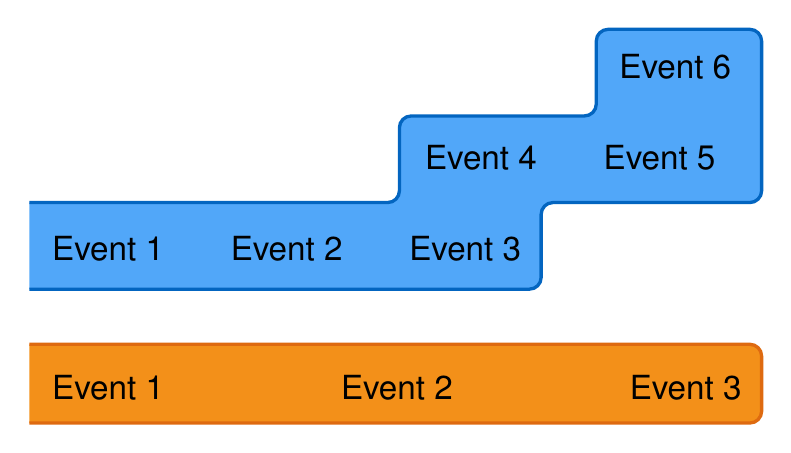
\begin{tikzpicture}[node distance=.6cm]

\path[c1, very thick, rounded corners=.15cm] (-1,-.45) -| ++(9.3,1) -- ++(-9.3,0);
\node (e11) at (0,0) {\large Event 1};
\node (e12) [right = 2cm of e11] {\large Event 2};
\node (e13) [right = 2cm of e12] {\large Event 3};

\path[c2, very thick, rounded corners=.15cm] (-1,1.25) -| ++(6.5,1.1) -| ++(2.8,2.2) -| ++(-2.1,-1.1) -| ++(-2.5,-1.1)  -- ++(-4.7,0);
\node (e1) [above = 1.2cm of e11] {\large Event 1};
\node (e2) [right = of e1] {\large Event 2};
\node (e3) [right = of e2] {\large Event 3};
\node (e4) [above = of e3, xshift=.2cm] {\large Event 4};
\node (e5) [right = of e4] {\large Event 5};
\node (e6) [above = of e5, xshift=.2cm] {\large Event 6};

\end{tikzpicture}

\end{document}